\section{Problem 1: Yang Pulang Membawa Laptopnya}
\label{sec:problem_1}

\subsection{Identifikasi Masalah}
Pada arsitektur sistem terdistribusi kebencanaan BNPB, lonjakan volume data dari berbagai jenis bencana yang mengalir bersamaan menyebabkan batas kapasitas vertikal (\textit{vertical scaling ceiling}) pada basis data tunggal tercapai. Penyimpanan tunggal menjadi \textit{I/O bottleneck} sekaligus menjadi \textit{single point of failure}. Ketika sistem mencoba membagi penyimpanan ke beberapa mesin, timbul dua permasalahan mendasar, yakni sebagai berikut.

\begin{enumerate}
    \item \textbf{Ketimpangan Beban Penyimpanan (\textit{Storage Skew \& Hotspotting}):} Kejadian gempa bumi secara alami tidak terdistribusi secara merata di seluruh ruang geografi, melainkan terkonsentrasi pada zona subduksi dan sesar tektonik aktif. Jika data dipartisi berdasarkan kriteria wilayah administratif atau sumber agensi saja, satu unit penyimpanan akan menanggung seluruh beban penulisan sementara unit lainnya menganggur.
    \item \textbf{Kegagalan Node dan Kehilangan Data (\textit{Node Loss \& Volume Wipe}):} Dalam sistem terdistribusi yang berjalan pada perangkat keras komoditas atau lingkungan fisik terpisah, node dapat mengalami kegagalan permanen, seperti pada skenario persoalan. Jika data hanya disimpan pada satu unit tanpa replikasi, rusaknya node tersebut mengakibatkan hilangnya catatan bencana secara permanen (\textit{catastrophic data loss}).
    \item \textbf{Reorganisasi Kapasitas Dinamis (\textit{Dynamic Rebalancing}):} Ketika node pengganti dimasukkan ke dalam kluster, sistem harus mampu mendistribusikan kembali data dan beban penulisan ke node baru tersebut secara dinamis tanpa mengharuskan pemadaman kluster (\textit{zero downtime rebalancing}).
\end{enumerate}

\vspace{1em}

\noindent Dalam literatur sistem terdistribusi, persoalan ini mencakup konsep \textbf{\textit{Database Sharding and Partitioning}}, \textbf{\textit{Partition Skew and Hotspots}}, \textbf{\textit{Fault Tolerance through Cross-Node Data Replication}}, \textbf{\textit{Consistent Hashing}}, serta \textbf{\textit{Graceful Degradation and Partial Availability}} sebagaimana dirumuskan pada Teorema CAP (mempertahankan ketersediaan penulisan dan pembacaan dengan status \textit{partial} saat terjadi partisi jaringan atau kegagalan node)~\cite{kleppmann2017designing,karger1997consistent,brewer2000towards,gilbert2002brewer}.

\vspace{1em}

\subsection{Rancangan Solusi dan Mekanisme}
Untuk menyelesaikan permasalahan ini, tim telah merancang arsitektur penyimpanan kanonis terpartisi menggunakan PostgreSQL Sharding dengan Consistent Hashing dan Replikasi Lintas Node yang dikelola langsung oleh layanan Aggregator (Gambar~\ref{fig:p1_sharding}). Berikut ini adalah penjelasan tambahan terkait solusi.

\begin{enumerate}
    \item \textbf{Cincin Hash Konsisten (\textit{Consistent Hash Ring}):} Penentuan lokasi shard untuk setiap kejadian bencana (\textit{HazardEvent}) dilakukan menggunakan fungsi hash SHA-256 64-bit \textit{big-endian} terhadap atribut identitas unik \texttt{hazard\_id}. Cincin konfigurasi memetakan 64 node virtual (\textit{vnodes}) per shard logis, menghasilkan sebaran kunci yang seragam dan meminimalkan pergeseran data saat terjadi penambahan atau pengurangan shard~\cite{karger1997consistent}.
    \item \textbf{Penempatan Asimetris Lintas Node (\textit{Asymmetric Cross-Node Placement}):} Kluster penyimpanan terdiri dari tiga shard logis (\texttt{shard-1}, \texttt{shard-2}, \texttt{shard-3}) dengan faktor replikasi dua ($RF=2$). Untuk mencegah kegagalan ganda pada satu host, pasangan primer (\textit{primary}) dan replika (\textit{replica}) tidak boleh berada pada node fisik yang sama:
    \begin{itemize}
        \item Node \texttt{aqua}: menampung \texttt{shard-1} (\textit{primary}) dan \texttt{shard-3-r1} (\textit{replica}).
        \item Node \texttt{ruby}: menampung \texttt{shard-2} (\textit{primary}) dan \texttt{shard-1-r1} (\textit{replica}).
        \item Node \texttt{akane}: menampung \texttt{shard-3} (\textit{primary}) dan \texttt{shard-2-r1} (\textit{replica}).
    \end{itemize}
    Dengan konfigurasi ini, tidak ada satu node pun yang menampung 100\% data kanonik (maksimum beban primer adalah sepertiga atau 33,33\% per node).
    \item \textbf{Mekanisme Penulisan dan Toleransi Kegagalan Terdegradasi:} Penulisan dilakukan secara konkuren menuju unit primer dan replika dari shard pemilik data. Transaksi penulisan dinyatakan berhasil jika minimal satu unit berhasil menyimpan data (\textit{degraded write availability}). Unit yang gagal dihubungi ditandai sebagai tertinggal (\textit{stale units}), dan sinkronisasi berkala latar belakang (\texttt{SyncShardReplicas}) akan memulihkan data yang tertinggal (\textit{anti-entropy reconciliation}).
    \item \textbf{Kueri Terpencar-Kumpul (\textit{Scatter-Gather Query}) dan Paginasi Deterministik:} Pembacaan yang melintasi seluruh lokasi penyimpanan (seperti membaca 50 event terbaru lintas jenis bahaya atau kueri Audit API) dieksekusi secara paralel menuju seluruh unit primer yang aktif (atau fallback ke replika bila primer mati)~\cite{hohpe2003enterprise}. Hasil dari tiap unit digabungkan dan diurutkan secara deterministik berdasarkan \texttt{(ingested\_at ASC, hazard\_id ASC)} menggunakan \textit{keyset cursor} berbasis base64url.
    \item \textbf{Penanganan Jawaban Parsial (\textit{Partial Response Guarantee}):} Bila salah satu node mati dan replikanya belum selesai menyinkronkan seluruh baris, API tidak mengembalikan kesalahan status 500 atau \textit{hanging request}, melainkan mengembalikan seluruh data yang berhasil dijangkau disertai penanda eksplisit [\texttt{"partial": true}] dan daftar unit yang tidak dapat dihubungi (\texttt{"unavailable\_units"}).
    \item \textbf{Penyeimbangan Ulang Daring (\textit{Online Cluster Rebalancing}):} Saat node baru ditambahkan, fungsi \texttt{RebalanceCluster} membangun cincin hash baru, memigrasikan rekaman yang berpindah kepemilikan, dan menghapus salinan \textit{stale} hanya setelah penulisan pada tujuan baru terkonfirmasi persisten.
\end{enumerate}

\begin{figure}[htbp]
    \centering
    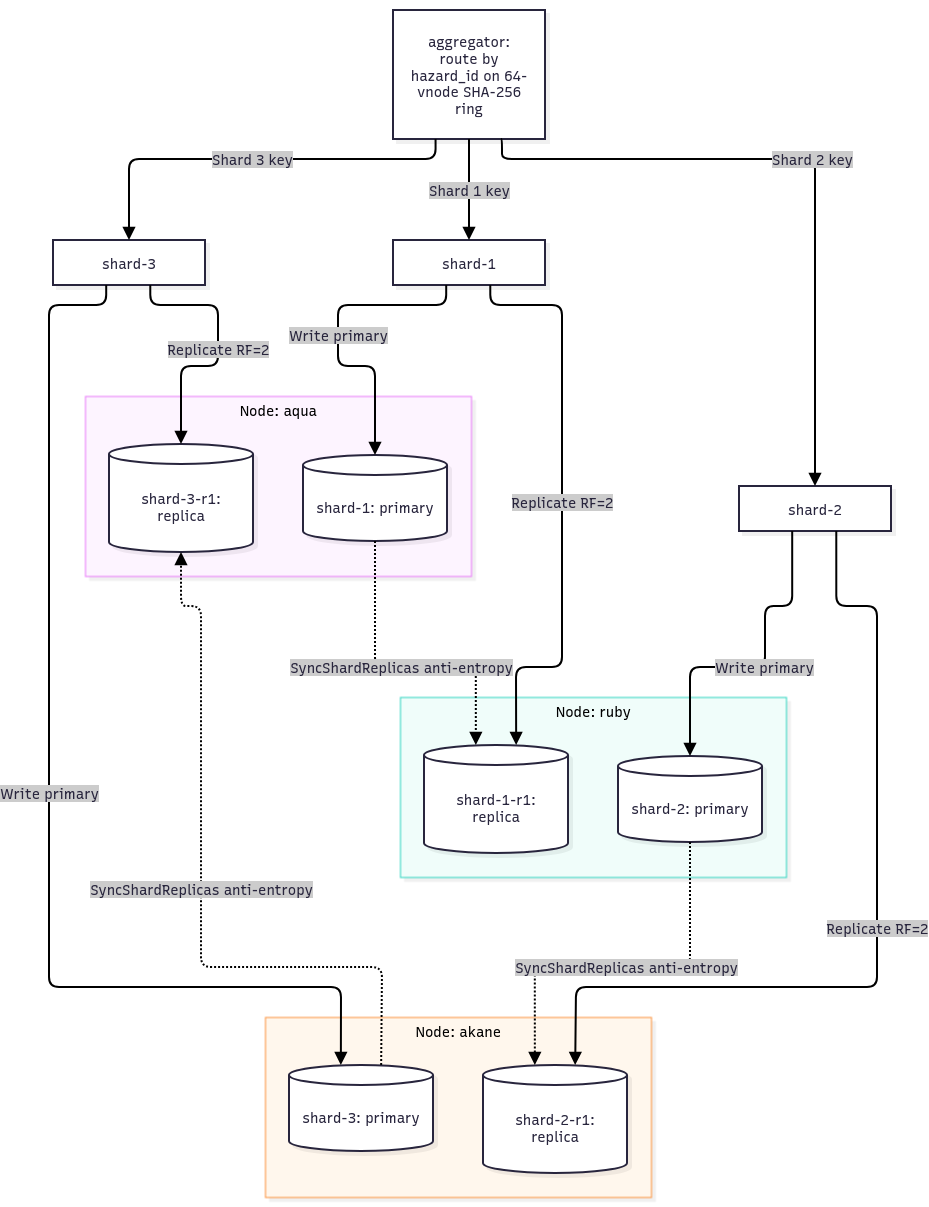
\includegraphics[width=0.72\textwidth, height=0.68\textheight, keepaspectratio]{figures/shard.drawio.png}
    \caption{Skema \textit{Consistent Hashing} 64-vnode, Penempatan Asimetris Lintas Node ($RF=2$), dan Sinkronisasi \textit{Anti-Entropy} pada Problem~1.}
    \label{fig:p1_sharding}
\end{figure}

\vspace{1em}

\subsection{Alasan Keputusan dan Trade-Off}
Dalam menentukan strategi pemartisian data pada kriteria 2, dievaluasi tiga alternatif pendekatan menggunakan dataset acuan 709 rekaman historis.

\begin{footnotesize}
\begin{xltabular}{\textwidth}{p{2.8cm} c c c c X}
\caption{Perbandingan Strategi Penempatan Data dan Ketahanan Skew} \label{tab:p1_placement_comparison} \\
\toprule
\textbf{Strategi} & \textbf{Katalog (709)} & \textbf{Skew} & \textbf{Spike (200)} & \textbf{Spike Skew} & \textbf{Hasil Evaluasi} \\
\midrule
\endfirsthead

\multicolumn{6}{l}{\textit{\footnotesize Lanjutan Tabel \ref{tab:p1_placement_comparison}}} \\
\toprule
\textbf{Strategi} & \textbf{Katalog (709)} & \textbf{Skew} & \textbf{Spike (200)} & \textbf{Spike Skew} & \textbf{Hasil Evaluasi} \\
\midrule
\endhead

\bottomrule
\endfoot

\textbf{ConsistentHash (\texttt{hazard\_id}, 64 vnodes)} & 239 / 234 / 236 & \textbf{1.011} & 60 / 75 / 65 & \textbf{1.125} & \textbf{Dipilih.} Sebaran beban sangat merata, kebal terhadap anomali geografis maupun lonjakan agensi hulu. \\
\midrule
RegionHash (\texttt{area\_name}) & 336 / 48 / 325 & 1.422 & 0 / 0 / 200 & 3.000 & \textbf{Ditolak.} 100\% rekaman gempa Jawa Barat menumpuk pada satu shard, memicu \textit{write hotspot}. \\
\midrule
AgencyPartition (\texttt{source}) & 0 / 703 / 6 & 2.975 & 0 / 200 / 0 & 3.000 & \textbf{Ditolak.} Volume BMKG mendominasi total data, melumpuhkan shard tunggal penampung BMKG. \\
\end{xltabular}
\end{footnotesize}

\noindent \textit{Trade-off} utama dari pemilihan \texttt{hazard\_id} adalah bahwa kueri analitik berbasis rentang waktu atau agensi harus melakukan pemindaian paralel (\textit{scatter-gather}) ke seluruh shard, dibanding langsung mengarah ke satu shard target. Namun, dengan batasan waktu baca (\textit{read timeout}) sebesar 2500 ms dan eksekusi paralel menggunakan Go \textit{goroutines}, latensi tambahan terukur hanya berkisar antara 10--25 ms, yang dinilai sebagai kompromi yang sangat menguntungkan untuk perlindungan dari bahaya \textit{write bottleneck}.

\vspace{1em}

\subsection{Batasan yang Disadari}
Implementasi solusi pada Problem 1 menyadari beberapa batasan teknis:
\begin{enumerate}
    \item \textbf{Konsistensi Replikasi Asinkron:} Sinkronisasi replika yang tertinggal (\textit{anti-entropy}) dieksekusi secara periodik latar belakang. Selama jendela propagasi tersebut, replika berada dalam kondisi konsistensi bertahap (\textit{eventual consistency}) sebelum rekonsiliasi selesai.
    \item \textbf{Ambang Batas Kehilangan Node:} Arsitektur dirancang bertahan terhadap kehilangan satu node ($N-1$). Kehilangan dua node penyimpanan secara bersamaan pada waktu yang sama melebihi faktor replikasi ($RF=2$), sehingga shard yang kehilangan kedua salinannya tidak dapat dijangkau dan memicu respons [\texttt{partial: true}].
    \item \textbf{Overhead Jaringan Scatter-Gather:} Pemanggilan lintas node menambah jumlah koneksi TCP pada kluster. Beban ini dimitigasi dengan penggunaan \textit{connection pool} terkelola dan \textit{bounded timeout}.
    \item \textbf{Kendala Sinyal \texttt{meta.degraded} dan Kejelasan Status pada Dasbor:} Pada layanan Aggregator, atribut \texttt{meta.degraded} menggabungkan dua pemicu berbeda yang sama-sama bersifat lokal per pod (\textit{process-local}), yakni kesehatan sumber hulu dari \texttt{status.\allowbreak Tracker} (mencakup \texttt{BMKG}, \texttt{PVMBG}, dan \texttt{Coastal}, sedangkan sumber \texttt{WILDFIRE} belum tercakup) serta kondisi penyimpanan parsial dari hasil \textit{scatter-gather} terakhir (\texttt{Storage\allowbreak Degraded\allowbreak Status}). Pada konfigurasi 3~replika Aggregator di belakang \textit{Service} terbagi beban, replika \textit{standby} yang tidak memegang \textit{leader lease} menyetel status hulu lokalnya tetap sehat, sehingga saat hulu terganggu hanya pod pemegang \textit{lease} yang melaporkan \texttt{meta.degraded = true}. Di sisi hilir, penggabungan \texttt{partial\_\allowbreak data = partial || degraded} pada \texttt{dashboard-consumer} juga sempat menimbulkan kendala ambiguitas pada tampilan awal antarmuka web (terlihat pada Gambar~\ref{fig:p1_dashboard_partial}, ketika kedua kondisi disatukan ke satu pil \texttt{PARTIAL / DEGRADED} dan lencana \texttt{INCOMPLETE} tanpa membedakan penyebab gangguan ataupun menampakkan apakah aliran Kafka langsung masih aktif). status \texttt{status.\allowbreak degraded} ditampilkan sebagai peringatan kritis merah (\texttt{DEGRADED} beserta \texttt{partial\_\allowbreak reason}), status \texttt{status.\allowbreak partial\_\allowbreak data} tanpa \texttt{degraded} ditampilkan sebagai peringatan kuning (\texttt{PARTIAL DATA} beserta daftar unit \texttt{unresponsive}), disertai indikator umur \textit{event} Kafka terbaru (\texttt{last\_\allowbreak kafka\_\allowbreak event\_at}) dan durasi degradasi (\texttt{stale\_\allowbreak since} relatif terhadap \texttt{generated\_at} server).
\end{enumerate}

\vspace{1em}

\subsection{Bukti Penyelesaian}
Bukti keberhasilan penyelesaian Problem 1 dibuktikan secara empiris melalui pengujian live pada kluster 3-node:
\begin{enumerate}
    \item \textbf{Pemuatan Katalog Gempa Historis (Kriteria 1 \& 2):} Dataset 709 kejadian bencana dimuat ke dalam kluster. Sebaran data terdistribusi secara seimbang: node \texttt{aqua} menampung 239 primer dan 236 replika, node \texttt{akane} menampung 236 primer dan 234 replika, serta node \texttt{ruby} menampung 234 primer dan 239 replika. Tidak ada node yang memuat seluruh data (maksimal 33,71\% primer). Rasio ketimpangan beban (\textit{skew ratio}) terukur sebesar 1.011 pada kondisi normal dan 1.125 pada kondisi simulasi lonjakan gempa.
    \item \textbf{Kueri Lintas Seluruh Shard dengan Paginasi (Kriteria 3):} Eksekusi endpoint \texttt{GET /internal/audit/events} berhasil mengambil 51.792 rekaman lintas seluruh shard melalui 52 halaman paginasi berurutan deterministik \texttt{(ingested\_at, hazard\_id)} tanpa duplikasi baris.
    \item \textbf{Ketahanan Terhadap Penghapusan Node / Wipe-Node (Kriteria 4):} Dilakukan simulasi pemadaman node \textit{worker} non-\textit{control-plane} \texttt{ruby} (\texttt{store-ruby-0}: \texttt{bnpb\_shard\_2} primer dan \texttt{bnpb\_shard\_1\_r1} replika) disertai pengosongan tabel penyimpanan (\texttt{TRUNCATE TABLE hazards, dlq\_messages}) serta uji partisi jaringan 35~detik pada \texttt{akane}. Selama partisi berlangsung, Audit API tetap menjawab HTTP~200 dengan penanda eksplisit \texttt{"partial": true} dan daftar \texttt{"unavailable\_units": ["shard-2-r1", "shard-3"]}.
    \item \textbf{Pemulihan dan Skalabilitas Node Baru (Kriteria 5 \& 6):} Setelah \texttt{store-ruby-0} dipulihkan dalam kondisi kosong, prosedur \texttt{SyncShardReplicas} menyinkronkan ulang 100\% data dari \texttt{store-akane-0} (\texttt{bnpb\_shard\_2\_r1}) dan \texttt{store-aqua-0} (\texttt{bnpb\_shard\_1}) secara otomatis di latar belakang dalam 57~detik (\texttt{shard-1=20.362}, \texttt{shard-2=20.511}, \texttt{shard-3=23.714}) tanpa menghentikan operasi baca maupun tulis. Pengecekan via \texttt{GET /internal/audit/checksum} pascapemulihan menghasilkan nilai SHA-256 yang utuh untuk seluruh 64.588~rekaman (\texttt{"partial": false}) serta mengembalikan ketahanan $RF=2$ terhadap kehilangan satu node berikutnya.
    \item \textbf{Dasbor Analitik Real-Time (Kriteria 7):} Dasbor analitik berbasis web berhasil menampilkan grafik deret waktu per jenis bahaya, agregasi tingkat keparahan, dan sebaran wilayah secara tepat. Saat simulasi pemadaman node berlangsung, dasbor tetap dapat diakses dan menampilkan lencana peringatan \texttt{PARTIAL DATA} secara transparan (Gambar~\ref{fig:p1_dashboard_partial}).
\end{enumerate}

\begin{figure}[H]
    \centering
    {\setlength{\fboxsep}{0pt}\color{gray!50}\fbox{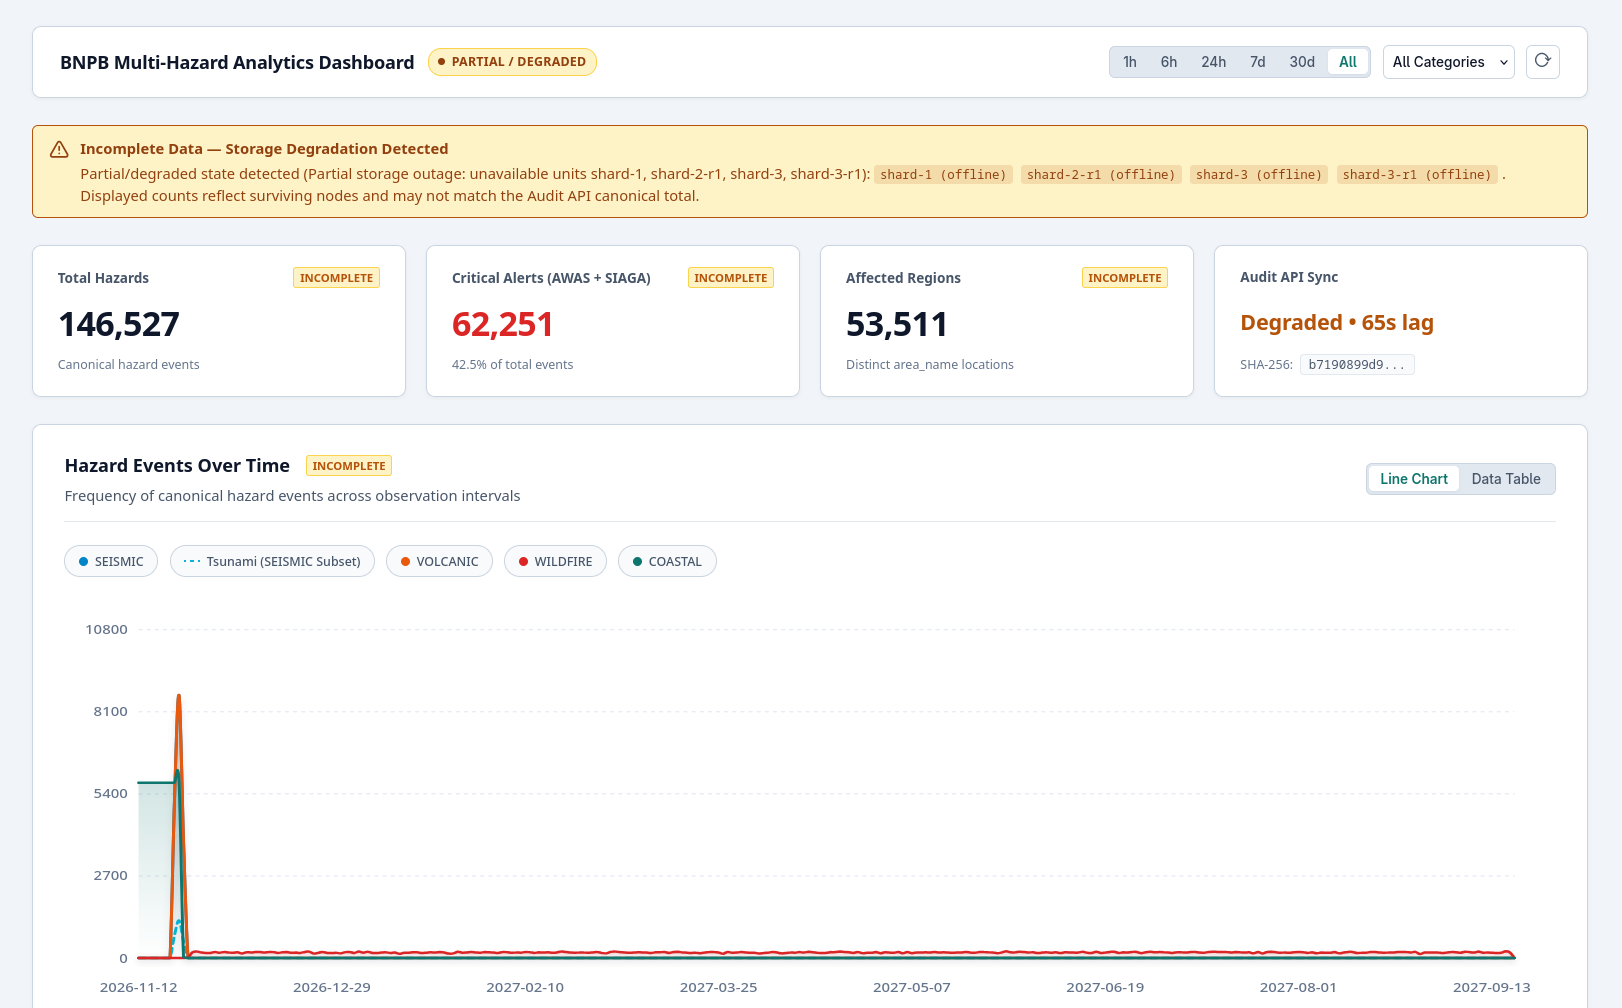
\includegraphics[width=0.92\textwidth]{figures/dash-consumer.png}}}
    \caption{Tangkapan layar antarmuka web \textit{BNPB Multi-Hazard Analytics Dashboard} (\texttt{/dashboard}) saat mendeteksi gangguan penyimpanan parsial, menampilkan peringatan \texttt{PARTIAL / DEGRADED}, lencana \texttt{INCOMPLETE}, status Audit API SHA-256, dan grafik deret waktu.}
    \label{fig:p1_dashboard_partial}
\end{figure}

\vspace{1em}

\subsection{Jawaban atas Butir ``Di Laporan''}
Berikut disajikan jawaban ringkas dan terstruktur atas pertanyaan pada spesifikasi tugas besar.
\begin{enumerate}
    \item \textbf{Identifikasi Persoalan dan Konsep Literatur:} Persoalan yang dihadapi adalah keterbatasan kapasitas node tunggal, ketimpangan distribusi beban geografis (\textit{data skew}), dan hilangnya data akibat musnahnya node penyimpanan. Dalam literatur sistem terdistribusi, konsep yang diterapkan adalah \textbf{\textit{Database Sharding}}, \textbf{\textit{Consistent Hashing}}, \textbf{\textit{Cross-Node Asymmetric Replication}}, dan \textbf{\textit{Graceful Degradation}}~\cite{kleppmann2017designing,karger1997consistent,gilbert2002brewer}.
    \item \textbf{Mekanisme Penentuan Lokasi Data dan Perubahan Dinamis:} Data dipetakan ke unit shard berdasarkan fungsi \texttt{SHA-256(hazard\_id)} pada cincin hash 64-vnode. Saat node bertambah atau berkurang, \texttt{ConsistentHashRing} memetakan ulang hanya pecahan kunci yang relevan ($\approx 1/N$ kunci), sementara proses rekonsiliasi \texttt{RebalanceCluster} mentransfer data secara inkremental tanpa mengunci tabel.
    \item \textbf{Perbandingan Alternatif Penempatan Data:} Dibandingkan terhadap \textit{Region-based Hash} (\texttt{hash(area\_name)}) dan \textit{Agency-based Partitioning} (\texttt{hash(source)}). Hasil pengukuran empiris menunjukkan kedua alternatif tersebut menghasilkan rasio ketimpangan ekstrem sebesar 3.000 saat terjadi lonjakan gempa regional, sedangkan \textit{ConsistentHash by hazard\_id} mempertahankan rasio seimbang pada 1.125.
    \item \textbf{Jaminan Konsistensi per Endpoint (Kondisi Normal dan Saat Node Hilang):}
    \begin{itemize}
        \item \texttt{POST /api/v1/field-reports} (alias \texttt{POST /field-reports}): Menjamin \textit{at-least-once durable staging} ke topik Redpanda \texttt{bnpb.field-reports} (\texttt{RequiredAcks: RequireAll}) sebelum mengembalikan \texttt{202 Accepted}. Persistensi ke penyimpanan kanonis bersifat \textit{eventual consistency} secara asinkron melalui konsumer Aggregator (dengan deduplikasi \texttt{(source, source\_ref\_id)}). Saat satu node penyimpanan hilang, penulisan kanonis tetap tersedia melalui unit replika yang bertahan ($RF=2$, \textit{degraded write availability}).
        \item \texttt{GET /api/v1/hazards}, \texttt{GET /api/v1/hazards/\{id\}}, dan \texttt{GET /internal/hazards}: Pada kondisi normal menjamin konsistensi pembacaan \textit{read committed} per \textit{shard} dengan membaca unit primer non-\textit{stale} (\textit{scatter-gather} paralel atau pencarian \textit{O(1)} via \texttt{?id=}). Saat satu node mati, pembacaan otomatis beralih ke unit replika (\textit{eventual consistency} selama jendela sinkronisasi \textit{anti-entropy}) dan ketidaktersediaan unit penyimpanan selama \textit{scatter-gather} langsung menandai \texttt{meta.degraded = true} beserta header \texttt{X-Storage-Partial: true} dan \texttt{X-Unavailable-Units}; bahkan bila kedua salinan suatu \textit{shard} tidak terjangkau, endpoint tetap merespons HTTP~200 dengan data tersisa dan daftar \texttt{unavailable\_\allowbreak units}, alih-alih HTTP~500.
        \item \texttt{GET /internal/audit/events}, \texttt{/checksum}, \texttt{/location}, dan \texttt{/unprocessed}: Pada kondisi normal menjamin pengurutan deterministik \texttt{(ingested\_at ASC, hazard\_id ASC)} dan \textit{checksum} SHA-256 \textit{byte-exact} terhadap seluruh unit primer. Saat satu node mati, jawaban tetap lengkap melalui replika. Bila sebagian unit tidak terjangkau, \texttt{/events}, \texttt{/checksum}, dan \texttt{/unprocessed} tetap mengembalikan HTTP~200 disertai \texttt{"partial": true} dan \texttt{unavailable\_units}, sedangkan \texttt{/location} mengembalikan \texttt{503} (bukan \texttt{404} palsu) apabila \textit{shard} pemilik tidak dapat dihubungi agar tidak keliru menyimpulkan rekaman hilang.
        \item \textbf{Dasbor Analitik (\texttt{GET /dashboard}, \texttt{GET /api/analytics}):} Menjamin \textit{near real-time eventual consistency} melalui proyeksi Kafka yang diselaraskan secara berkala terhadap Audit API; pada kondisi gangguan parsial, menyajikan \textit{snapshot} terakhir dengan penanda eksplisit \texttt{"partial\_data": true}.
    \end{itemize}
    \item \textbf{Perhitungan Agregasi Dasbor dan Penandaan Data Tidak Terjangkau:} Layanan \texttt{dashboard-consumer} tidak mengakses PostgreSQL secara langsung karena diblokir oleh \texttt{NetworkPolicy} (\texttt{isolate-storage-strict}). Sebaliknya, dasbor memproyeksikan event dari topik \texttt{bnpb.hazard-events} secara \textit{update-aware} di memori (memperbarui metrik per jenis bahaya, tingkat keparahan, dan wilayah tanpa penggandaan) serta melakukan rekonsiliasi delta via \texttt{GET /internal/audit/events?since=...} dan validasi \texttt{GET /internal/audit/checksum} ke Aggregator setiap 5~detik (serta sinkronisasi penuh tiap 300~detik atau saat \textit{checksum} menyimpang), di mana Aggregator mengeksekusi \textit{scatter-gather} lintas seluruh \textit{shard}. Apabila respons Audit atau Aggregator menyertakan \texttt{"partial": true}, header \texttt{X-Storage-Partial: true}, \texttt{meta.degraded = true}, atau gagal dihubungi, dasbor mempertahankan tampilan terakhir yang sah, menyetel \texttt{status.\allowbreak partial\_\allowbreak data = true} (dan \texttt{status.degraded = true} bila sumber atau sinkronisasi terdegradasi) beserta \texttt{status.\allowbreak partial\_\allowbreak reason} serta \texttt{stale\_\allowbreak since}, lalu menampilkan pemisahan peringatan \texttt{DEGRADED} versus \texttt{PARTIAL DATA} dan indikator kesegaran aliran Kafka (\texttt{last\_\allowbreak kafka\_\allowbreak event\_at}) di antarmuka web.
\end{enumerate}
